\section{Evaluation}
\label{sec:evaluation}

Our evaluation answers the following questions:
\begin{compactenum}
\item Can the system rapidly deploy new data-sets? 
\item What is the read latency, and does it scale with data size and nodes? 
Also what is the impact on it during a new data deployment?
\end{compactenum}

We use a simulated data-set as well as production data for two
user-facing features: ``People You May Know'' (PYMK,
c.f.~Figure~\ref{fig:pymk}) and ``Viewers of this profile also
viewed'' (collaborative filtering or CF,
c.f.~Figure~\ref{fig:browsemaps}). All tests were run on Linux~2.6.18
machines with Dual CPU (each having 64-bit 8~cores running at~2.67 GHz),
24~GB RAM and 6~RAID~10 drives. We used Community Edition
version 5.0.27 and MyISAM storage engine for all our MySQL tests.

Since the read-only storage engine relies on OS page cache, we gave 
it only 4 GB JVM heap. Similarly since MyISAM uses a special key cache
for index blocks and the page cache for data blocks, we chose the same
4 GB for \emph{key\_buffer\_size}. We start by describing the data-sets in detail.

\begin{compactitem}
\item \emph{Random data-set}. The key is a long between
0 and a varying number. The value is a fixed 1024 bytes size random
string. 
\item \emph{PYMK data-set}. Users are presented with recommendations
of other users whom they might know and would like connect with. This
is presented as a store where they key is the logged in user's id
while the value is a list of integer recommended ids and a float
score. Figure~\ref{distribution} shows the value size distribution for
this store. 
\item \emph{Collaborative filtering (CF) data-set}. This product shows
other viewed profiles in the same session as the visited member's
profile. The value is a list of 2 integer identifiers, a string
indicating the entity type, and a float score.
Figure~\ref{distribution} shows the value size distribution for CF. 
\end{compactitem}

\begin{figure}
  \centering
    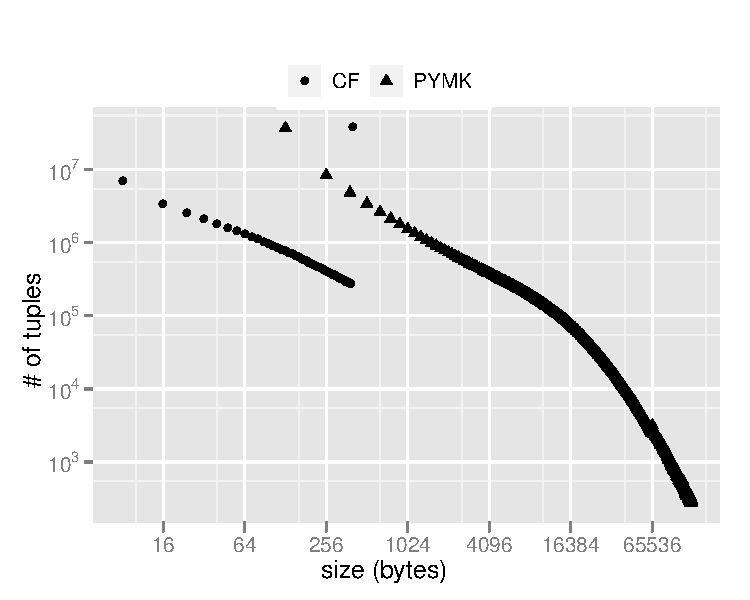
\includegraphics[scale=0.55]{images/data_distribution.pdf}
  \caption{Value size distributions for PYMK and CF. The abrupt stop
is due to the cap on the number of recommendations we provide.}
  \label{distribution}
\end{figure}

\subsection{Build times}

One of the important goals of \projectname{} is rapid data deployment,
which means the build and push phase must be fast. Push times are
entirely dependent on available network bandwidth, so we focus on
build times.
 
The build time in case of \projectname's Hadoop workflow includes the
time to generate the chunk mapping in the map phase, shuffle the data,
and finally, in the reduce phase, emit the store files. The number of
mappers and reducer are kept fixed so as to have same amount of
parallelism. This also resulted in fixed number of chunks being
generated.

In case of MySQL, the build time is the completion time of the
\sql{LOAD DATA INFILE} command on an empty table. This ignores the 
time it took to convert the data to TSV and copy it over to the MySQL 
node. Some optimizations to make MySQL faster include increasing the 
MySQL bulk insert buffer size and the MyISAM specific sort buffer 
size to 256 MB each and also delaying the re-creation of the index 
to a latter time by running \sql{ALTER TABLE...DISABLE KEYS} statement 
before the load. 

Besides the B$^{+}$ tree structure built inside MySQL, we build our
own B$^{+}$ tree structure tailored to Hadoop. Instead of generating
chunk files in every reducer step, we generate a B$^{+}$ tree. This
tree contains of a single data file, similar to the chunk data file,
and a set of index files corresponding to every level of the tree. The
bulk loading of the tree is done in blocks (of size~$b$); that is, the
system first finishes the lower level's block and only then
initializes a block at the next level. The system applies this rule
recursively for every level as the sorted elements stream through.
This bulk loading approach is efficient in that it does not require
buffering any values in memory and the system can directly write to
the level-based index files. 

Figure~\ref{build} shows the build time as we increased the size of
the input data-set. The block size~$b$ for the B$^{+}$ was set to~340,
which was chosen as the keys were 12~bytes long (8~byte MD5 and 4~byte
offset) and the system page size is~4096 bytes. This meant the best
block size would be approximately $4096/12 \sim 340$. 

As is clearly evident, MySQL exhibits extremely slow build times since it buffers
the changes to the index before flushing it to disk. Also due to the
incremental changes required to the index on disk, MySQL does around
1.4 times more I/O than our implementation. This number would amplify 
if we had bulk loaded into a non-empty table. The optimized B$^{+}$, 
on the other hand, performs well for small sizes but deviates at larger 
input sizes due to the extra I/O required: extra disk writes for the 
higher levels of the tree are necessary. For a fixed block size, 
the extra disk writes are linear with the number of tuples. 
Further, we do not discuss the serving latency for the custom B$^{+}$ tree 
implementation since it is sensitive to machine-specific block size~$b$.
% Should we mention that this implementation also had file size
% problems  = multiple small HDFS files, but can be solved in future work 
% by using array based single file

\begin{figure}
  \centering
    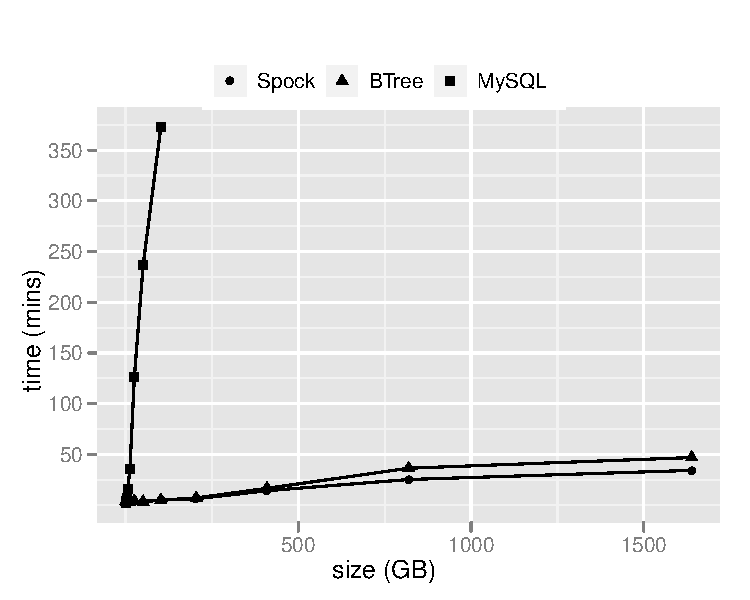
\includegraphics[scale=0.55]{images/build.pdf}
  \caption{The time to complete the build for varying input data size. We terminated the MySQL test early due to prolong data load time} 
  \label{build}
\end{figure}

\subsection{Read latency}

Besides rapid data deployments, the read latency must be acceptable
and the system must scale with the number of nodes. For the random
data-set, we used 10~million requests with simulated values following
a uniform distribution. For the PYMK and CF data-set, we use a
snapshot of member activity for one high traffic day.

We first try to measure how fast the index can get paged into the OS's
page cache. We ran tests on a 100~GB random data-set on a single node
and report the median latency after swap for a continuous stream of 
uniformally distributed requests. For MySQL, we created a view 
on an existing table, bulk loaded into a new table and swapped the view 
to the new table without stopping the requests. Similarly for our 
storage engine we used the complete data-pipeline, described in Section
~\ref{sec:read_only:data_cycle}, to swap new data. The single node was 
configured to have just one partition and one chunk per chunk bucket. 
We also compared the binary and interpolation search algorithms for 
read-only storage engine.  

Figure~\ref{search} shows the median latency versus time since the swap.
MySQL system starts with a very high median latency due to the un-cached
index and falls slowly to the stable 1.4 ms mark. On the other hand, our
storage engine has a relatively cached index since our swap retrieves index
files after the data files. Binary search initially starts with a high 
median latency compared to interpolation, but the slope of the line 
is steeper. This is because binary search did an average of 8~lookups 
thereby touching more parts of the index; interpolation search, on the 
other hand, performs an average of only 1~lookup. While this results 
in an initial low read latency, it comes at the expense that much of the 
index is uncached in the long run. Our production systems are currently 
running binary search due to this faster cache warming process. All numbers 
presented henceforth for read-only storage engine use binary search.  

\begin{figure}
  \centering
    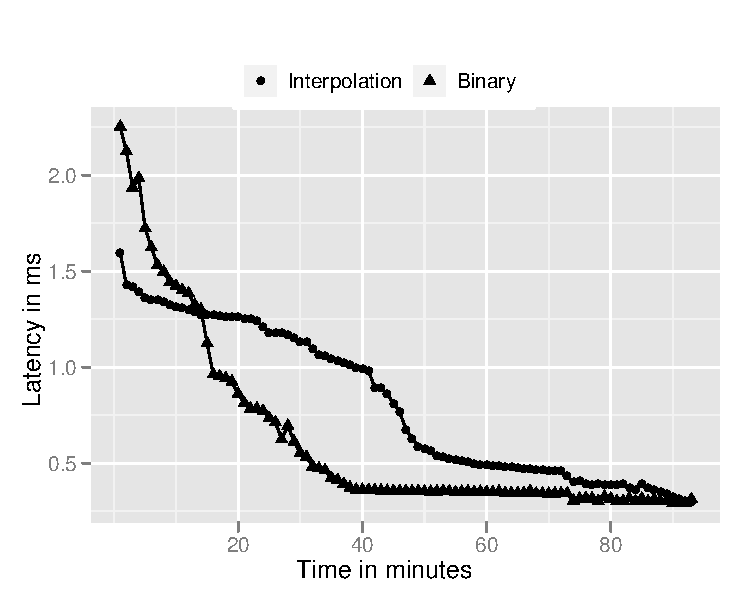
\includegraphics[scale=0.55]{images/search_1node.pdf}
  \caption{Single node median read latency taken at 1 minute intervals since the swap. The slope of the graph shows the rate of cache warming}
  \label{search}
\end{figure}

Figure~\ref{mysql:search} also shows a comparison of \projectname's
performance to MySQL on the same 100~GB data-set for varying 
throughput after warming up the cache. We increased the client 
side throughput till the actual throughput stopped increasing. 
As is clearly evident our implementation scales to around twice
the amount of queries per second while maintaining the median latency. 

\begin{figure}
  \centering
    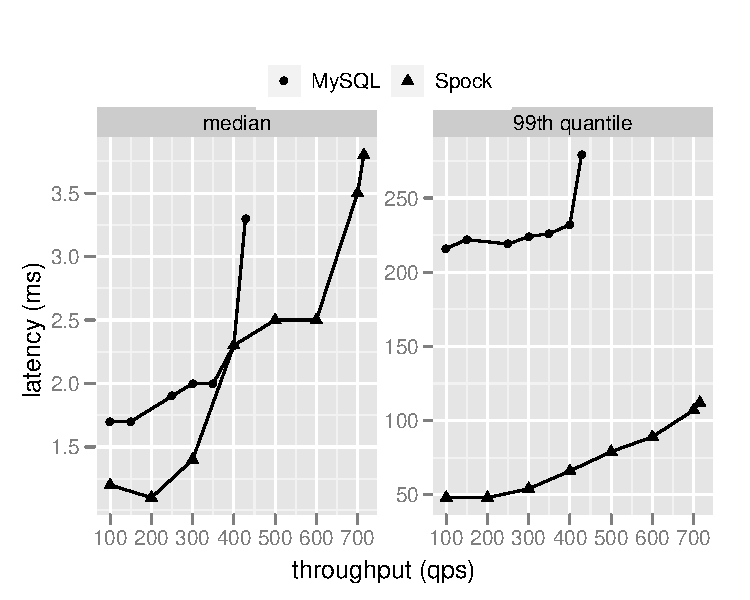
\includegraphics[scale=0.55]{images/mysql_vs_read.pdf}
  \caption{Single node read latency after warming up the cache for a while. This figure shows the change in latency as we vary the client throughput}
  \label{mysql:search}
\end{figure}

To test whether the system scales well with the number of nodes, we
present read latency numbers for the same random data-set but spread
over 16~machines and $N$=1. The data was fetched by \projectname{} at a steady
rate bound by the network; we saturated the 1~Gbit line between HDFS
and \projectname{} nodes. The read tests were run for both uniform as well as
zipfian distribution using YCSB~\cite{ycsb}, an open-source framework 
for benchmarking cloud data serving systems, with number of clients fixed
at 100 threads. The Zipfian distribution ensures that the hot elements are 
queried together since that simulates the general site visiting patterns 
of most websites~\cite{zipf}. We also observed that the separate node
running the client was never a bottleneck since most of the time was
spent in retrieving the data.
Figure~\ref{16search} shows the overall client side median latency while varying 
the data-set sizes. The hotness of a few keys naturally aids cachability, 
thereby exhibiting an overall lower latency for zipfian compared to 
the uniform distribution. 

\begin{figure}
  \centering
    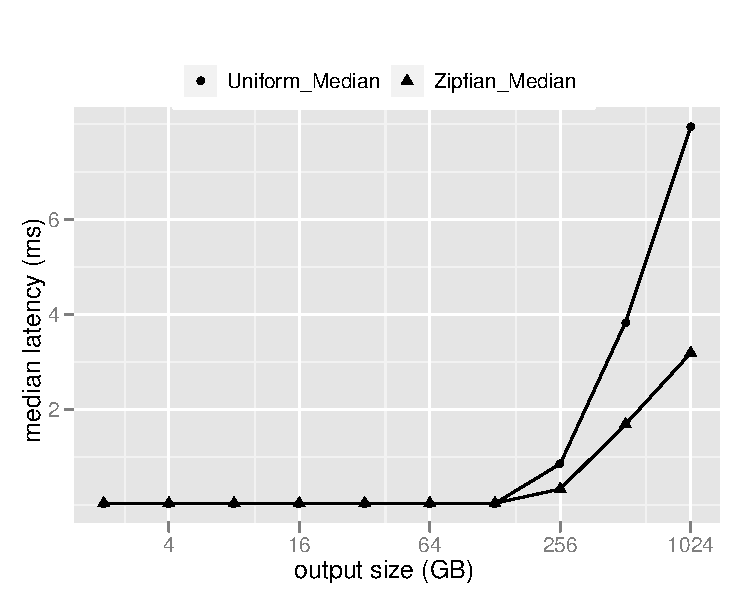
\includegraphics[scale=0.55]{images/search_16node.pdf}
  \caption{Client side median latency with varying data size for 2 request distributions, on a 16 node cluster. We stopped after 1 TB due to disk space requirements on the cluster}
  \label{16search}
\end{figure}

Finally, Table~\ref{tab:production_statistics} shows some of the statistics 
for our largest cluster. Figure~\ref{production} shows the PYMK and CF average
read latencies, over a 5 minute sliding window, on a node from this cluster. Both
the stores use $N$=2 and $R$=1. In particular we highlight the latency difference 
before and after a data swap. Our corresponding client side latency has the same
trend along with the extra network overhead. CF has a higher latency than that of 
PYMK primarily because of the larger data size.

\begin{figure*}
  \centering
    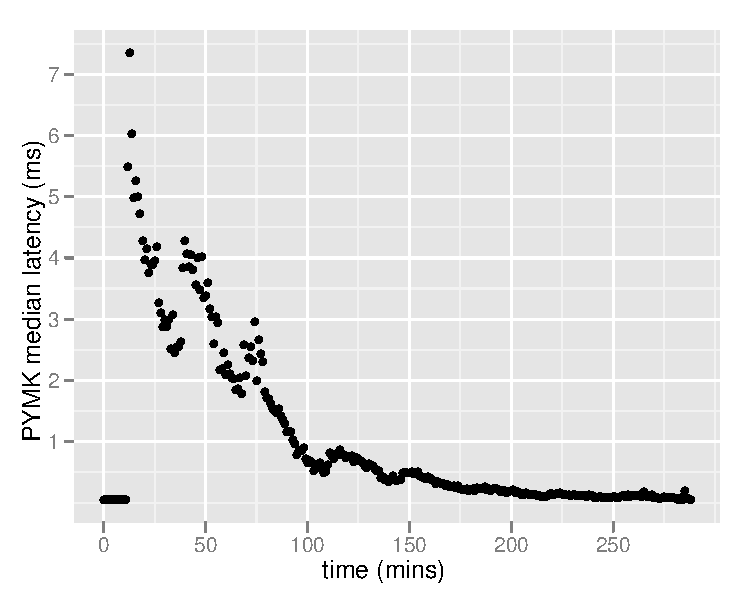
\includegraphics[scale=0.55]{images/pymk_search.pdf}
    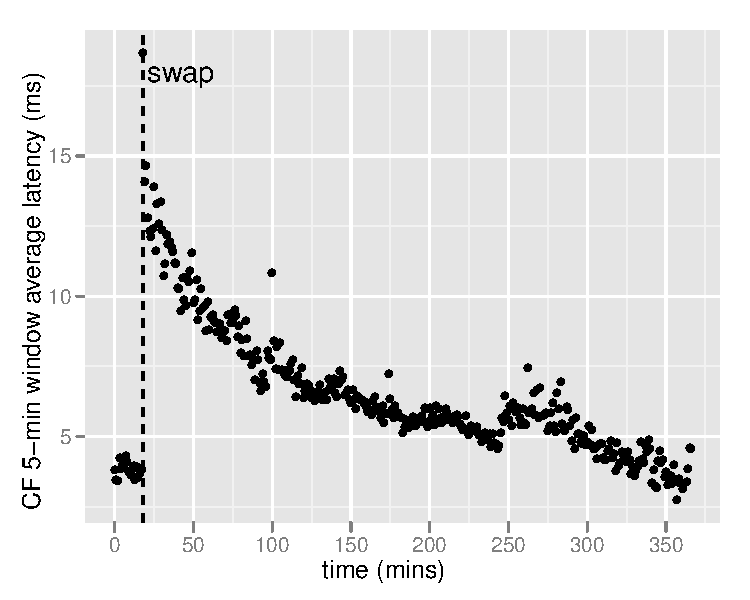
\includegraphics[scale=0.55]{images/browsemap_search.pdf}
  \caption{5 minutes sliding average read latency across all server nodes on our largest cluster over time. The dotted line shows the time when the new data-set was swapped in}
  \label{production}
\end{figure*}

\begin{table}
\begin{center}
	\begin{tabular} { | l | l | }
	\hline
	Total data size per node &	940 GB			\\ 
	Current active data to memory ratio &	11.7:1		\\
	\hline
	Total number of stores &	110 	\\
	Max store size  &		320 GB	\\
	Min store size &		46 KB	\\
	Max number of store swaps per day & 66	\\
	\hline
	\end{tabular}
\end{center}
	\caption{Statitics of our largest read-only cluster at \linkedin{}}
 	\label{tab:production_statistics}
\end{table}


